\documentclass{beamer}
\usepackage{ulem}
\mode<presentation>{} 
\title{Rails 3: A Quick Introduction}
\author{Eliza Brock  \\@elizabrock  \\github:elizabrock}
\date{\today}
%\includeonlyframes{current}
\AtBeginSection[]{} % for optional outline or other recurrent slide
\mode<presentation>
{ \usetheme{Malmoe} }
\begin{document}

\begin{frame}
\titlepage
\end{frame}

\section{Introduction}
\begin{frame}
\frametitle{First Things First}
% Every tutorial ever written for rails is now wrong.
\pause
\begin{itemize}
\item rails blog
\end{itemize}
\end{frame}

\begin{frame}
\frametitle{First Things First}
% Every tutorial ever written for rails is now wrong.
\begin{itemize}
\item \sout{rails blog}
\item rails new blog
\end{itemize}
\end{frame}

\section{Up and running}
\begin{frame}
\frametitle{Installing rails}
\begin{semiverbatim}
\$ rvm use ree@rails3demo --create

\$ gem install rails
\end{semiverbatim}

\pause
Installs:\\
\begin{tabular}{l l l}
activesupport-3.0.0 & builder-2.1.2 & i18n-0.4.1 \\
activemodel-3.0.0 & rack-1.2.1 & rack-test-0.5.5 \\
rack-mount-0.6.13 & tzinfo-0.3.23 & abstract-1.0.0 \\
erubis-2.6.6 & actionpack-3.0.0 & arel-1.0.1 \\
activerecord-3.0.0 & activeresource-3.0.0 & mime-types-1.16 \\
polyglot-0.3.1 & treetop-1.4.8 & mail-2.2.6.1 \\
actionmailer-3.0.0 & rake-0.8.7 & thor-0.14.1 \\
railties-3.0.0 & bundler-1.0.0 & rails-3.0.0 \\
\end{tabular}
\end{frame}

\begin{frame}
\frametitle{Highpoint \#1}

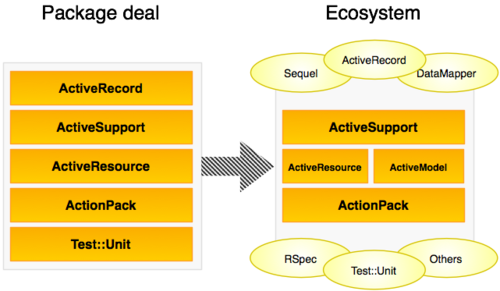
\includegraphics[width=4in]{omgbloglol_rails3_packaging.png}

http://omgbloglol.com/post/344792822/the-path-to-rails-3-introduction
\end{frame}



\begin{frame}
\frametitle{Starting a new project with 'rails new'}

\begin{itemize}
\item Arguments! Lots of arguments!
\item \begin{semiverbatim}\$ rails new railsdemo -d mysql -T -J \end{semiverbatim}

\item Yields a new project, railsdemo, using mysql without prototype or test::unit
\end{itemize}
\end{frame}


\begin{frame}
\frametitle{Installing rspec with bundler}

Let's add rspec to our project, shall we?
\pause

In the Gemfile, add:
\begin{semiverbatim}
group :development, :test do

     gem 'rspec-rails', '2.0.0.beta.22'
     
end
\end{semiverbatim}
\pause
Then just run bundler!

\begin{semiverbatim}
\$ bundle install
\end{semiverbatim}

\pause

Done!
%Explain why this is awesome
\end{frame}

\begin{frame}
\frametitle{One Last Little Thing}

\begin{semiverbatim}
rails generate rspec:install
\end{semiverbatim}

\end{frame}



\section{Bit of customization}
\begin{frame}
\frametitle{Say hello to generators}
Hi!
\pause

Just add a bit of config to config/application.rb:

\begin{semiverbatim}
config.generators do |g|
      
      g.test\_framework :rspec, :fixture => true, :views => false
end
\end{semiverbatim}

\end{frame}

\begin{frame}
\frametitle{Drum roll please...}
\begin{semiverbatim}
\$ rails generate scaffold tutorials
\end{semiverbatim}
\pause

yields:


\begin{semiverbatim}
      ...
      
      create    app/models/tutorial.rb
      
      invoke    rspec
      
      create      spec/models/tutorial\_spec.rb
      
      create      spec/fixtures/tutorials.yml
      
       route  resources :tutorials
      
      invoke  scaffold\_controller
      
      create    app/controllers/tutorials\_controller.rb
      
      ...
\end{semiverbatim}
%lookie there, we're getting rspec generated for us!
\end{frame}

\section{Other High Points}

\begin{frame}
\frametitle{Other High Points:}

\begin{itemize}
\item Performance
\item Syntactic Sugar
\item AREL
\item XSS
\end{itemize}

\end{frame}

\section{Looking Forward: Rails 3.1}
\begin{frame}
\frametitle{The Future Is... Not Quite Here}

\begin{itemize}
\item Ruby 1.9
\pause
\item Deprecations from 3.0 will be gone in 3.1!
\pause
\item Fibers/Rendering magic
\end{itemize}
\end{frame}


\section{The Rails 3 Way}
\begin{frame}
\frametitle{Some Resources}
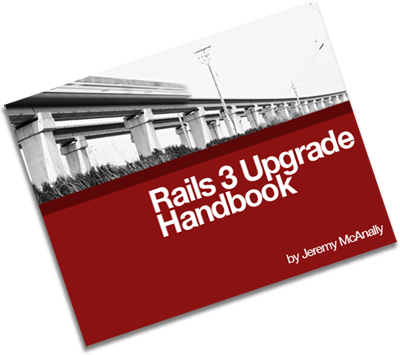
\includegraphics[width=2in]{rails3upgradehandbook.png}
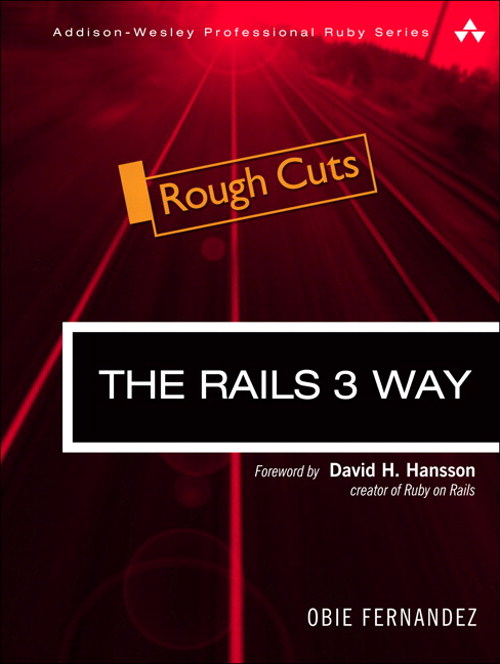
\includegraphics[width=1.75in]{rails3way.jpeg}  
\end{frame}


\end{document}